
\section{Preliminaries}\label{sec::1.1}

%In the following, we will assume a sequence of $n$ independent and identically distributed (iid) random variables (R.V.) that we will write, for convenience, in the form of $\{X_i\}=X_1,X_2,\dots ,X_n$. Note that the iid assumption will be relaxed in \hyperref[sec::3]{Chapter \textbf{\ref{sec::3}}}.

In the following, a sequence of independent and identically distributed (iid) random variables are assumed and written in the form $\{X_n\}_{n\in\mathbb{N}}$. The $X_i$'s share a common cumulative distribution function (df) $F$. The iid assumption will be relaxed in \hyperref[sec::3]{Chapter \textbf{\ref{sec::3}}}.


%\addcontentsline{toc}{subsection}{Statistical Tools}
\subsection*{Statistical Tools}

Let $X_{(i)} $ denote the $i$-th ascending order statistic,

\begin{equation} \label{ordereds}
X_{(1)}\leq X_{(2)}\leq \ldots \leq X_{(n)},
\end{equation}
assuming $n$ observations.
One order statistic is of particular interest, the \emph{maximum} $X_{(n)}$
\begin{equation} \label{max}
X_{(n)}:=\displaystyle{\max_{1\leq i\leq n}}X_i,
\end{equation}
while the \emph{minimum} $X_{(1)}$ can be defined it with respect to the maximum operator

\begin{equation}\label{min}
X_{(1)}:=\displaystyle{\min_{1\leq i\leq n}}X_i=- \displaystyle{\max_{1\leq i\leq n}}(-X_i).
\end{equation}
This text will focus on maxima but it is important to keep in mind that the analysis made in the following can be extended to minima through relation (\ref{min}).

Furthermore, we can retrieve the distribution of $X_{(n)}$. By definition,
\begin{equation}\label{maxdist}
\begin{aligned}
\text{Pr}\{X_{(n)}\leq x\} & \ =\text{Pr}\{X_1 \leq x, \ldots, X_n \leq x\} \\ &\stackrel{(\independent)}{=}\text{Pr}\{X_1\leq x\}\dots\text{Pr}\{X_n\leq x\} \\
&\ =F^n(x),
\end{aligned}
\end{equation}
where the independence $(\independent)$  follows directly from the iid assumption of the sequence $\{X_i\}$.


%Finally, remark that we included some concepts of statistical convergence in \hyperref[convconc]{Appendix \ref{convconc}}, as it will often appear in the text.


\subsection*{First Definitions and Theorems : Motivations}
\theoremstyle{definition}
\begin{definition}[Distributions of same type]\label{similardf} We say that two dfs $G$ and $G^*$ are of the \emph{\textbf{same type}} if, for constants $a>0$ and $b$ we have
	\begin{equation}\label{simm}
	G^*(az+b)=G(z), \ \ \ \ \ \ \forall z.
	\end{equation}
\end{definition}
This means that the distributions only differ in location and scale. 
This concept will be useful later in the text to derive the three different families of extreme value distributions which come from other distributions that are of the \emph{same type}.


\paragraph*{Principles of stability :}
% course slides 18 coles 
Amongst the principles about EVT that will be covered during this text, EVT will be highly influenced by the principles of \emph{stability}. It states that a model should remain valid and consistent whatever choices are made on the structure of this model.
For example, if we propose a model for the annual maximum temperatures and another for the 5-year maximum temperatures, the two models should be mutually consistent since the 5-year maximum will be the maximum of 5 annual maxima. Similarly, in a Peaks-Over-Threshold setting (presented in \hyperref[sec::2]{Chapter \textbf{\ref{sec::2}}}), a model for exceedances over a high threshold should remain valid for exceedances of higher thresholds. 



\begin{definition}[Max-stability] \label{maxstab}
	\emph{From \cite{leadbetter_extremes_1983} or \cite{resnick_extreme_1987}}, we say that a distribution $G$ is \emph{\textbf{max-stable}} if, for each $n\in\mathbb{N}$ we have	
	\begin{equation}
	G^n(a_nz+b_n)=G(z), \ \ \ \ \ \ \ n= 1,2,\dots ,
	\end{equation}
	for appropriate normalizing constants $a_n>0$ and $b_n$.
\end{definition}
In other words, taking powers of $G$ results only in a change of location and scale. This concept will be closely connected with the fundamental limit law for extreme values that we will present in the \hyperref[sec:extrtypethm]{next Section}.
However, the power of max-stable processes is often used in a multivariate setting, whereas we will focus on univariate sequences. Refer for example to \citet{ribatet_spatial_2015} for an introduction on max-stable processes.
%\emph{Min-stability} can easily be found by complement, see for instance \citet[pp.23]{ reiss_statistical_2007} for an example.


A fundamental concept of EVT is the concept of \textbf{degenerate} dfs. We recall that the df of a random variable is said to be \emph{degenerate} if it assigns all probability to a single point.
We illustrate this by the construction of the well-known \emph{Central Limit Theorem} (CLT) that we will state below and which concerns the sample mean $\bar{X}_n=n^{-1}\sum_{i=1}^nX_i$. We know from the Weak Law of Large Numbers that  $\bar{X}_n$ will converge \emph{almost surely} to the true mean $\mu$ (see\footnote{\hyperref[convconc]{Appendix \textbf{\ref{convconc}}} can be useful for a relevant short review of main concepts of convergence.} \hyperref[wlln]{Theorem \textbf{\ref{wlln}}}). and thus in distribution, that is to a non-random single point, i.e. to a \emph{degenerate} distribution 

\begin{equation*}
\text{Pr}\big\{\bar{X}_n\leq x\big\}= \begin{cases}
\ 0, \ \ \ \ \ \ \ \ \ \ \ \ x<\mu; \\
\ 1, \ \ \ \  \ \ \ \ \ \ \ \ x\geq \mu. 
\end{cases}
\end{equation*}
This is not useful, in particular for inferential purposes. 
%\vspace{-.7cm}
%\begin{center}\small{[\textit{The reader may refer to \hyperref[convconc]{Appendix \ref{convconc}} for a short review of main concepts of convergence}]}
%\end{center}

For this reason, CLT aims at finding a non-degenerate limiting distribution for $\bar{X}_n$, after allowing for normalization by sequences of constants. We will state it in its most basic form :

\begin{exe}[Central Limit Theorem] 
	Let $\{X_i\}$ be a sequence of $n$ iid random variables with $E(X^2_i)<\infty$. Then, $\text{as} \ n\rightarrow\infty$,
	
	\begin{equation*}
	\sqrt{n}(\bar{X}_n-\mu)\stackrel{d}{\longrightarrow}N(0,\sigma^2),
	\end{equation*}
	where $\mu=E(X_i)$ and $\sigma^2=V(X)>0$.
\end{exe}

Then, by making a proper choice of some normalizing constants, $\mu$ and $\sqrt{n}$ (as location and scale parameters respectively), we find the non-degenerate normal distribution in the limit for the empirical mean $\bar{X}_n$ provided $X_i$ has a nonzero variance and finite second moment. 

With the same logic, we find for the distribution of maximum order statistics $X_{(n)}$ 
\begin{equation}
\displaystyle{\lim_{n \to \infty}}\text{Pr}\big\{X_{(n)}\leq x\big\}=\displaystyle{\lim_{n \to \infty}}\text{Pr}\big\{X_i\leq x\big\}^n=\begin{cases}
\ 0, \ \ \ \ \ \ \ \ \ \ \  \ \ \ F(x)<1; \\ 
\ 1, \ \ \ \ \ \ \ \ \ \ \ \  \ \ F(x)=1,
\end{cases}
\end{equation}
which is also a degenerate distribution.

Whereas the CLT dealt with the sample mean, EVT also aims to find a non-degenerate distribution in the limit of the maximum $X_{(n)}$ by means of normalization. %We will see how it works in details in the following section.


\section{Extremal Types Theorem : Extreme Value distributions}\label{sec:extrtypethm}


Introduced by \cite{fisher_limiting_1928}, later revised by \cite{gnedenko_sur_1943} and streamlined by \cite{de_haan_regular_1970}, the \emph{extremal types theorem} is important for its applications in EVT. Let $\{X_i\}$ be a sequence of iid random variables with df $F$. It states the following :  

\begin{theorem}[Extremal Types] \label{extthm}
 If there exist sequences of normalizing constants $a_n>0$, $b_n\in\mathbb{R}$ and a non-degenerate limiting distribution $G$ such that 
	\begin{equation} \label{exttheom}
	\displaystyle{\lim_{n \to \infty}}\text{\emph{Pr}}\Big\{ a_n^{-1}(X_{(n)}-b_n)\leq z\Big\}=F^n(a_nz+b_n)
	= G(z), \ \ \ \ \ \ \ \ \forall z\in\mathbb{R},
	\end{equation}
then $G$ has the same type as one of the following distributions : 

\begin{equation}\label{gumb}
\boxed{\textbf{\text{I}}}\ : \qquad G_{1}(z)= 
\exp\Big\{-e^{-z}\Big\}, \ \ \quad \quad \ \ -\infty<z<\infty.    
\end{equation}


\begin{equation} \label{frech}
\boxed{\textbf{\text{II}}} \  :  \quad G_{2,\alpha}(z)=
\begin{cases}
\ 0, \ \ \ \ \ \ \ \ \ \ \ \qquad \quad \ \ \ \ \ \ \ \quad \ \ z\leq 0; \\
\ \exp\Big\{-z^{-\alpha}\Big\}, \ \ \ \quad \ \quad \ \ \ z>0.    
\end{cases}
\end{equation}

\begin{equation} \label{weib}
\ \ \boxed{\textbf{\text{III}}} \ :  \quad G_{3,\alpha}(z)=\begin{cases}
\ \exp\Big\{-\big(-z\big)^{\alpha}\Big\}, \quad \quad \   z<0;     \\
\  1, \ \ \ \ \ \ \qquad \quad \quad \ \ \ \ \ \ \ \ \  \   \quad z\geq 0,
\end{cases}
\end{equation}
for some parameter $\alpha>0$ in case II and III.
\end{theorem}

These are termed the \emph{standard extreme value distribution functions} and are differentiated by three types. Note that each real parameter $\alpha$ determines the type. \textbf{Type} $\boxed{\textbf{\text{I}}}$ is commonly known as the \emph{Gumbel} family while the \textbf{type} $\boxed{\textbf{\text{II}}}$  and \textbf{type} $\boxed{\textbf{\text{III}}}$ are known as the \emph{Fréchet} and the \emph{Weibull} families respectively. From the fact that $G$ is of the \emph{same type} as one of the three distribution, we can rescale these distributions by some normalizing parameters $a>0$ (scale) and $b$ (location), that is $G_{i,\alpha, a,b}(z)=G_{i,\alpha}\Big(\frac{z-b}{a}\Big)$ for $i=2,3$, and similarly for $G_1$ to obtain the \emph{full} EV distributions. %Note that $b$ will become the left endpoint of $G_{2,\alpha}$ and the right endpoint of $G_{3,\alpha}$.


This theorem considers an iid random sample, but it holds true even if the original scheme is no longer independent. We will present the stationary case in 
\hyperref[sec:statio]{Section \textbf{\ref{sec:statio}}}. Furthermore, we will see in \hyperref[sec:mda]{Section \textbf{\ref{sec:mda}}} that $F$ is in the \emph{domain of attraction} of $G$. %Now, let's find out if there exist a more convenient characterization of $G$.  %However, even the stationary assumption is often poor in practical applications (see for our applications in our case, the temperature....)\cite{gomes_bootstrap_2015} (see application...) but we will handle that in \hyperref[nstatio]{section \textbf{3.2}}. 


\subsection{Generalized Extreme Value Distribution}\label{sec:gevdistri}

\citet{von_mises_distribution_1936} showed that another representation is possible by taking the reparametrization $\xi=\alpha^{-1}$ of the extreme values dfs to obtain a continuous, unified model.

Hence, these three classes of extreme distributions can be expressed in the same functional form as special cases of the single three-parameter \textit{Generalized Extreme Value} (GEV) distribution 
\begin{equation} \label{gevgen}
G(z):=G_{\xi,\mu,\sigma}(z)\ =\text{exp}\ \Bigg\{-\bigg[1+\xi\bigg(\frac{z-\mu}{\sigma}\bigg)\bigg]_+^{-\xi^{-1}}\Bigg\}, \quad \ \ \xi\neq 0.
\end{equation}
where $-\infty<\mu,\xi<\infty$ and $\sigma>0$ with $(\mu,\sigma,\xi)$ being the three parameters of the model characterizing location, scale and shape respectively. We introduce the notation $y_+=\text{max}(y,0)$ to denote that (\ref{gevgen}) is defined on $\big\{z:1+\xi\sigma^{-1}(z-\mu)>0\big\}$. It ensures the term in the exponential function is negative, and the df converges to 1. It is important to note that this yields a vital condition for the GEV as it defines the endpoints from the three different characterizations of this distribution from the values of the shape 
parameter. %This will be detailed in the \hyperref[sec:gevdistri]{next Section}.

The GEV corresponds to the \emph{Fréchet} family (\ref{frech}) whenever $\xi>0$ and to the \emph{Weibull} family (\ref{weib}) as $\xi<0$.
When $\xi=0$, i.e. for the \emph{Gumbel} family (\ref{gumb}), the situation in (\ref{gevgen}) is not defined but is taken as the limit as $\xi\to 0$, leading to 

\begin{equation}\label{gevgen0}
G(z):=G_{\mu,\sigma}(z)=\ \exp \Bigg\{-\exp\bigg(\frac{z-\mu}{\sigma}\bigg)\Bigg\}, \qquad\qquad\qquad \ \ \xi=0.
\end{equation}

The shape parameter $\xi\in\mathbb{R}$ is called the \emph{extreme value index} (EVI) and is at the center of the analysis in EVT. It determines, in some degree of accuracy, the type of the underlying distribution. %Often, another parametrization based on $\alpha=\xi^{-1}$ is used in the literature to emphasize the fact that ... Hence, from this general definition of the GEV distribution (\ref{gevgen})-(\ref{gevgen0}), we can directly retrieve the \textbf{three principal types of EV distributions} from the value $\xi$ :

Following \cite{coles_introduction_2001}, we introduce an important theorem in Extreme Value Theory and that has many implications. This theorem states the following :

\begin{theorem}\label{max-gev} For any df $F$,
	
	\begin{equation}
	F \ \emph{\text{is \emph{max-stable}}}\ \Longleftrightarrow \ F \emph{\text{ is GEV}}.
	\end{equation}
\end{theorem}
Hence, any df that is \emph{max-stables} (see \hyperref[maxstab]{ Definition \textbf{\ref{maxstab}}}) is also GEV (\ref{gevgen})-(\ref{gevgen0}), and vice-versa. To gain interesting insights of the implications of this theorem, we think it is useful to give an informal proof but only for the "$\Leftarrow$" as the converse requires a significant mathematical background. By using max-stability (\hyperref[maxstab]{Definition \textbf{\ref{maxstab}}}) and \hyperref[max-gev]{Theorem \textbf{\ref{max-gev}}}, this "proof" also gives intuition for \hyperref[extthm]{Theorem \textbf{\ref{extthm}}}. 

\begin{proof}[\boxed{\emph{\textbf{Outline Proof}}}\nopunct ] of \textbf{Extremal Types} \hyperref[extthm]{Theorem \textbf{\ref{extthm}}} (and \hyperref[max-gev]{Theorem \textbf{\ref{max-gev}}}) :
	\vspace{-0.1cm}
\ \ \	\begin{itemize}
    \item	If $a_n^{-1}(X_{(n)}-b_n)$ has the GEV as limit distribution for large $n$ as defined in (\ref{exttheom}), then
	
	\begin{equation*} \label{gevproof1}
	\text{Pr}\Big\{ a_n^{-1}(X_{(n)}-b_n)\leq z\Big\}\approx G(z).
	\end{equation*}
	Hence for any integer $k$, since $nk$ is large, we have
	\begin{equation} \label{bigup}
	\text{Pr}\Big\{ a_{nk}^{-1}(X_{(n)k}-b_{nk})\leq z\Big\}\approx G(z).
	\end{equation}
	
	\item Since $X_{(n)k}$ is the maximum of $k$ variables having identical distribution as $X_{(n)}$,
	
	\begin{equation} \label{bigup1}
	\text{Pr}\Big\{ a_{nk}^{-1}(X_{(n)k}-b_{nk})\leq z\Big\}=\Big[\text{Pr}\big\{ a_{nk}^{-1}(X_{(n)}-b_{nk})\leq z\big\}\Big]^k,
	\end{equation}
	giving two expressions for the distribution of $X_{(n)}$, by (\ref{bigup}) and (\ref{bigup1}) :
	
	\begin{equation*}\label{gevproofl}
	\text{Pr}\{X_{(n)}\leq z\}\approx G\Big(a_n^{-1}(z-b_n)\Big) \ \ \ \ \text{and} \ \ \ \ \text{Pr}\{X_{(n)}\leq z\} \approx G^{1/k}\Big(a_{nk}^{-1}(z-b_{nk})\Big).
	\end{equation*}
	\item It follows that $G$ and $G^{1/k}$ are identical apart from location and scale coefficients. 
	Hence, $G$ is \emph{max-stable} and therefore GEV. This gives intuition of the \textbf{extremal 
	types} \hyperref[extthm]{Theorem \textbf{\ref{extthm}}}.
  \end{itemize}
\vspace{-.3cm}
\end{proof}
In words, it means that taking power of $G$ results only in a change of location and scale, and hence by recalling the expression of the distribution of $X_{(n)}$(\ref{maxdist}), it is possible to find the non-degenerate GEV in the limit for $X_{(n)}$. More technical details can be found in \citet{leadbetter_extremes_1983}.

%\vspace{-.5cm}
\subsubsection*{Density} 
The density of the GEV distribution (\ref{gevgen}), $g(z)=\frac{d G(z)}{dz}$ (since we have absolute continuity) can be expressed in two forms, as depicted in Table \ref{tab:gevdens}.

\begin{table}[!htb]
\centering\caption{Two cases for the \emph{density distribution} of the GEV}\label{tab:gevdens}
\begin{tabular}{c|c}

$\xi\neq 0$ &  $g(z)=\sigma^{-1}\bigg[1+\xi\bigg(\frac{z-\mu}{\sigma}\bigg)\bigg]_+^{-\frac{1}{\xi}-1}\exp\Bigg\{-\bigg[1+\xi\bigg(\frac{z-\mu}{\sigma}\bigg)\bigg]_+^{-\xi^{-1}}\Bigg\}$; \\
 \hline  \\
$\xi\to 0$ & $g(z)= \sigma^{-1}\exp\bigg\{-\bigg(\frac{z-\mu}{\sigma}\bigg)\bigg\}\exp\Bigg\{-\exp\bigg[-\bigg(\frac{z-\mu}{\sigma}\bigg)\bigg]\Bigg\}$. \\ 

\end{tabular}
\end{table}

We can now try to visually represent these three families. The following Figure \ref{gevdens} depicts the GEV, defined with respect to the value of the shape parameter $\xi$. 

\begin{figure}[!htb]
	\centering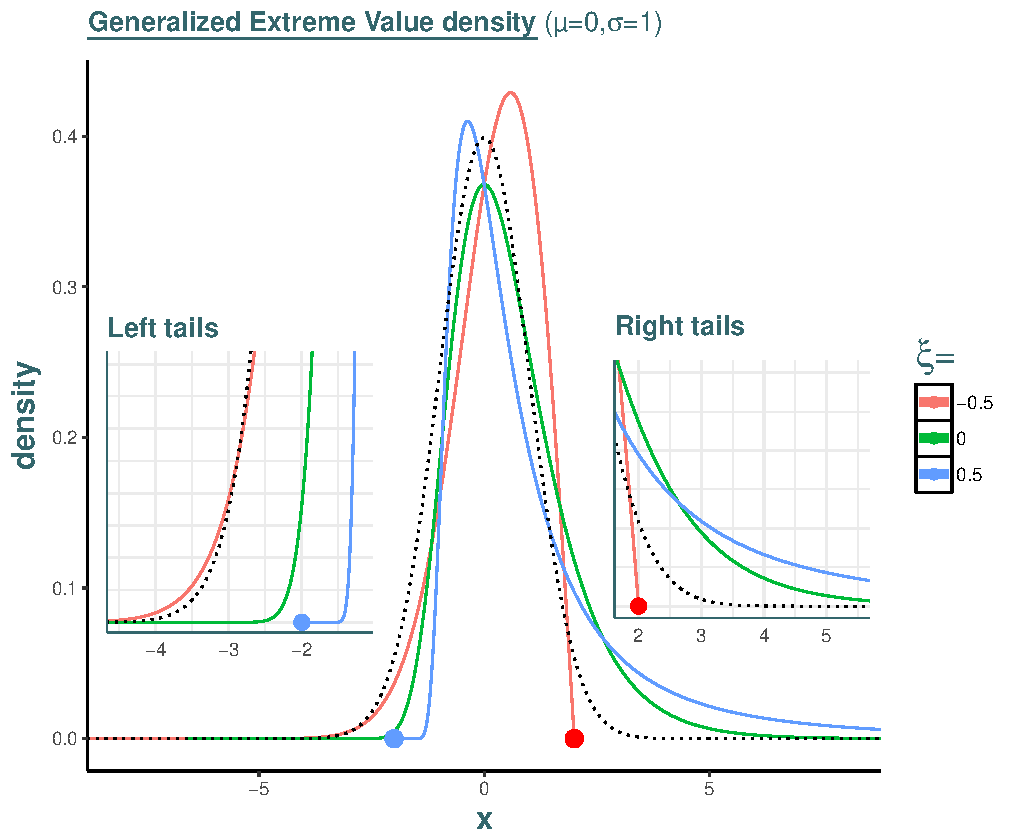
\includegraphics[width=0.8\linewidth]{gev3.pdf}\caption{GEV distribution with the normal as benchmark (dotted lines) and a zoom on the parts of interest to better visualize the behaviour in the tails. In green, we retrieve the Gumbel distribution ($\xi=0$). In red, we retrieve the Weibull-type ($\xi<0$) while in blue, we get the Fréchet-type ($\xi>0$). The endpoints for the Weibull and the Fréchet are denoted by the red and blue filled circles respectively. }\label{gevdens}
\end{figure}


It is important to point out that the location parameter $\mu$ does not represent
the mean as in the classic statistical view rather it represents the “center” of the distribution; and the scale parameter
$\sigma$ is not the standard deviation but does govern the “size” of the deviations around $\mu$. This can be visualized in Figure \ref{fig:gevdif} in \hyperref[app:fig]{Appendix \textbf{\ref{app:fig}}} where we show the variation of the GEV distribution when we vary these parameters\footnote{Moreover, a Shiny application has been built through the R package to visualize in the best way the influence of the parameters on this distribution. See intro of \hyperref[chap:introana]{Chapter \textbf{\ref{chap:introana}}} for an explanation on its use.}. We notice that the location parameter only implies a horizontal shift of the distribution, without changing its shape, and w see the influence of the scale parameter on the spread of the distribution around $\mu$. For example if $\sigma \nearrow$, then the density will appear more flat.  

In the following, we define the \emph{left} and the \emph{right} \emph{endpoint} of a particular df $F$ as respectively $_*x$ and $x_*$, by :
\begin{equation}\label{eq:endpoints}
_*x=\inf\{x\in\mathbb{R}:F(x)>0\}, \ \ \ \ \ \ \text{and} \ \ \ \ \  x_*=\sup\{x\in\mathbb{R}:F(x)<1\}.
\end{equation}
Note that the Gumbel distribution is unbounded. The Fréchet distribution has a finite left endpoint in $_*x=\mu-\sigma\cdot\xi^{-1}$ (blue circle in Figure \ref{gevdens}), and its upper endpoint is $+\infty$ while the Weibull distribution has a finite right endpoint in $x_*=\mu-\sigma\cdot\xi^{-1}$ (red circle in Figure \ref{gevdens}) and is unbounded in the left. This has serious impact on modeling. Since these endpoints are functions of the parameter values,  will see later in \hyperref[likgevintro]{Section \textbf{\ref{likgevintro}}} that it can make the likelihood computation unstable. We will particularly face this in the Bayesian \hyperref[sec::bayesian]{Chapter\textbf{ \ref{sec::bayesian}}}.
% For example,we when dealing with maximum temperatures it is intuitive to consider it is more probably bounded to the right than to left, meaning that a maximum temperature of 70°c is impossible, and hence a Weibull distribution will appear more frequently. 

\vspace{.15cm}
It can be useful to think not only about the
specific form of data or the distribution they will fit and its characteristics, but also about how to retrieve these specific distributions in practice. That is why we detail some examples of how to construct such EV distributions for the three types in concrete cases, playing with the appropriate choice of 
sequences $a_n$ and $b_n$ to retrieve the pertaining distribution family.
%\newline

\section{Applications : Examples of Convergence to GEV}\label{sec::appconcrete}

In real applications it is not easy to find the appropriate sequences, but it is useful to understand the concept of convergence to GEV by looking at some theoretical examples.


\subsection*{Convergence to Gumbel distribution}
The \textbf{Type}  $\boxed{\textbf{\text{I}}}$ or \textbf{Gumbel} distribution $G_1$ can be retrieved by considering, for example, an iid exponentially distributed sequence $\{X_j\}$ of $n$ random variables, that is $X_j\stackrel{iid}{\sim}Exp(\lambda)$ and taking the largest of these values, $X_{(n)}$, as defined earlier. By definition, if the $X_j$ have df $F$, then $F(x)=1-e^{-\lambda x}$ for $x>0$. Hence, our goal is to find non-random sequences $\{b_n\}$, $\{a_n>0\}$ such that 
\begin{equation}
\displaystyle{\lim_{n \to \infty}}\text{Pr}\Big\{ a_n^{-1}(X_{(n)}-b_n)\leq z\Big\}=G_1(z).
\end{equation}
Hence, we can easily find that
\begin{equation*}
\begin{aligned}
\text{Pr}\Big\{ a_n^{-1}(X_{(n)}-b_n)\leq z\Big\}
&=\text{Pr}\big\{X_{(n)}\leq b_n+a_nz\big\} \\ &=\Big[\text{Pr}\{X_1\leq b_n+a_nz\}\Big]^n \\
&=\Big[1-\exp\big\{-\lambda(b_n+a_nz)\big\}\Big]^n,
\end{aligned}
\end{equation*}
from the iid assumption of the random variables and their exponential distribution.
Hence, by choosing  the sequences $a_n=\lambda^{-1}$ and $b_n=\lambda^{-1}\log n$ and reminding that% $\displaystyle{\lim_{n \to \infty}}(1+\frac{x}{n})^n=\exp(x)$,


\begin{equation*}
\begin{aligned}
\Big[1-\exp\big\{-\lambda(b_n+a_nz)\big\}\Big]^n 
& = \Big[1-\frac{1}{n}e^{-z}\Big]^n %\ \ \ \ \ \ \ \ \ \ \ \ \ \ \ \ \ \ \ \ \ \ \ \ \ %\scriptsize\text{\underline{Recall:}} \ \ %\begin{adjustbox}{minipage=0.2\textwidth,precode=\dbox} \scriptsize\displaystyle{\lim_{n \to \infty}}\Big(1+\frac{x}{n}\Big)^n=\exp(x)
%\end{adjustbox}
%\boxed{\scriptsize\displaystyle{\lim_{n \to \infty}}\Big(1+\frac{x}{n}\Big)^n=\exp(x)} \\
& \stackrel{n\to\infty}{\longrightarrow} \exp(-e^{-z}):=G_1(z),
\end{aligned}
\end{equation*}
we find the so-called standard \emph{Gumbel} distribution in the limit. 
Note that the same can be retrieved with $X_j\stackrel{iid}{\sim}N(0,1)$ and with sequences $a_n=-\Phi^{-1}(1/n)$ and $b_n=1/a_n$. 

\vspace{.2cm}
Typically unbounded distributions, for example the Exponential and Normal, whose tails fall off exponentially or faster, will have the Gumbel limiting distribution for the maxima. They will have, in particular, medians (and other quantiles) that grow as $n\rightarrow\infty$ at the rate
of 'some power of' $\log n$. This is a typical example of light-tailed distribution (i.e., whose tails decay exponentially, as defined in \hyperref[app:tails]{Appendix \textbf{\ref{app:tails}}}).

\vspace{-.3cm}
\subsection*{Convergence to Fréchet distribution}

The \textbf{Type}  $\boxed{\textbf{\text{II}}}$ or \textbf{Fréchet type} (or \emph{Fréchet-Pareto}) distribution $G_2(x)$ has strong relations with the Pareto distribution and also the Generalized Pareto Distribution that will be presented in \hyperref[sec::2]{Chapter \textbf{\ref{sec::2}}}. These are distributions which are typically heavy- or fat-tailed (see \hyperref[app:tails]{Appendix \textbf{\ref{app:tails}}}).

%[Practical analysis of extreme values p.51]
Following \citet{beirlant_practical_1996}, when starting with a sequence $\{X_j\}$ of $n$ iid random variables following a \textit{basic} (or \textit{generalized} with scale parameter set to 1) Pareto distribution with shape parameter $\alpha\in (0,\infty)$, $X_j\sim Pa(\alpha$), we have that 

\begin{equation}
F(x)=1-x^{-\alpha}, \ \ \ \ \ \ \ \ \ \ \ \ \ \ x\in[1,\infty).
\end{equation}
Then, by setting appropriately $b_n=0$, we can write

\begin{equation*}
\begin{aligned}
-n\bar{F}(a_nz+b_n)
& =-n(a_nz+b_n)^{-\alpha} \\
& =\Big[F^{\leftarrow}(1-\frac{1}{n})\Big]^{\alpha}(a_n)^{-\alpha}(-z^{-\alpha}),
\end{aligned}
\end{equation*}
where we define the quantity $F^{\leftarrow}(t)=\inf\{x\in\mathbb{R}:F(x)\geq t\}$ for $t<0<1$ as the \emph{generalized inverse\footnote{from which we can retrieve $x_t=F^{\leftarrow}(t)$, the $t$-quantile of $F$. Even if we deal in this text only with continuous and strictly increasing df, we prefer consider \emph{generalized inverse}, for sake of generalization.} of F}.
Hence, it is easy to see that by setting $a_n=n^{1/\alpha}$ and keeping $b_n=0$, we have that 
\begin{equation*}
\text{Pr}\{a_n^{-1}X_{(n)}\leq z\}\rightarrow \exp (-z^{-\alpha}),
\end{equation*}
showing that for those particular values of the normalizing constants, we retrieve the Fréchet distribution in the limit of a basic Pareto distribution. The fact that $b_n$ is set to zero can be understood intuitively since for heavy-tailed distribution (see) such as the Pareto distribution, a correction for location is not necessary to obtain a non-degenerate limiting distribution, see \citet[pp.51]{beirlant_practical_1996}.
%[see p.28 memoire other si ft autre exemple]
More generally, we can state the more general following theorem :
\begin{theorem}[Pareto-type distributions] For the same choice of normalizing constants as above, i.e. $a_n=F^{\leftarrow}(1-n^{-1}))$ and $b_n=0$ and for any $x\in\mathbb{R}$, if
	\begin{equation}
	\begin{aligned}
	n[\bar{F}(a_nx)]= \frac{\bar{F}(a_nx)}{\bar{F}(a_n)}\rightarrow x^{-\alpha} ,&&&&&&&&&&&& \text{ n}\to\infty,
	\end{aligned}
	\end{equation}
	then we say that "\emph{$\bar{F}$ is of Pareto-type}" or, more technically, "\emph{$\bar{F}$ is regularly varying with index -$\alpha$}".
\end{theorem}

This theorem is interesting to get an understanding of the shape of the tails of this kind of distributions. 
We define the concepts of \emph{regularly varying functions}, together with \emph{slowly varying functions} in \hyperref[app:varying]{Appendix \textbf{\ref{app:varying}}}
%\citet[pp.51-54]{beirlant_practical_1996} and supported by 
%\citet[pp.49, 77-82]{beirlant_statistics_2006}.
%\citet[pp.75]{beirlant_statistics_2006} !!!!

\subsection*{Convergence to EV Weibull distribution}

The \textbf{type}  $\boxed{\textbf{\text{III}}}$ or \textbf{Weibull} family (?) of distributions $G_3(x)$ arises, for example, in the limit of $n$ iid uniform random variables $X_j\sim U[L,R]$ where $L$ and $R>L$ are both in $\mathbb{R}$  and denote respectively the Left and the Right endpoint of the domain of definition. We have by definition

\begin{equation*}
F(x)=\frac{x-L}{R-L}, \ \ \ \ \ \ \ \  \ \ x\in [L,R].
\end{equation*}
It is $0$ for $x<L$ and $1$ for $x>R$.
We assume we are in the general case, i.e. $[L,R]$ can be $\neq [0,1]$. When choosing $a_n=R$ and $b_n=(R-L)/n$, we find the unit Reversed Weibull distribution $We(1,1)$ in the limit 

\begin{equation*}
\begin{aligned}
\text{Pr}\{a_n^{-1}(X_{(n)}-b_n)\leq z\}
&=\text{Pr}\{X_{(n)}\leq b_n+a_nz\} \\
& = \bigg[1-\frac{R-b_n-a_nz}{R-L}\bigg]^n, \qquad\qquad L\leq b_n+a_nz\leq R \\ 
& = \Big(1+\frac{z}{n}\Big)^n\to e^z, \ \qquad \qquad\qquad  z\leq 0 \quad \text{and} \quad n>|z|.
\end{aligned}
\end{equation*}
 That is, the Weibull-type GEV with $\xi=-1$.
 This is a typical example of the maximal behavior for bounded random variables with
continuous distributions.


\subsection*{Conditions and Comments}

Intuitively, it stands to reason that the df $F$ needs certain conditions for the limit to exist in \hyperref[extthm]{Theorem \textbf{\ref{extthm}}}. There exists a \emph{continuity condition} at the right endpoint $x_*$ of $F$ which actually rules out many important distributions. For example, it ensures that if $F$ has a jump at its finite $x_*$ (e.g. discrete distributions), then $F$ cannot have a non-degenerate limit distribution as in (\ref{exttheom}). Examples are well documented in \citet[section 3.1]{embrechts_modelling_2011} for the Poisson, Geometric and Negative Binomial distributions. We cannot find a nondegenerate distribution in the limit for these distributions even after normalization, which limit the scope for applications of the Extremal Types \hyperref[extthm]{Theorem \textbf{\ref{extthm}}}. 

Let's finish by noting that it is actually not mandatory to find the normalizing sequences for inferential purposes.
We can ignore the normalizing constants in practical applications and fit directly the GEV in our set of maxima.
The estimated parameters $\mu$ and $\sigma$ will implicitly take the normalization into account, while the shape parameter $\xi$ is not affected. We will see more details about this at the beginning of \hyperref[sec::3]{Chapter \textbf{\ref{sec::3}}} for the stationary case, while methods to estimate $\big( \mu, \sigma,\xi\big)$ will be presented in \hyperref[sec::gevinfernce]{ Section \textbf{\ref{sec::gevinfernce}} } . Now let's characterize more precisely the distributions pertaining to the GEV.

\section{Maximum Domain of Attraction}\label{sec:mda}

The preceding results can be more easily summarized and obtained when considering \emph{maximum domain of attraction} (MDA). The term "\emph{maximum}" is typically used to make the difference with \emph{sum-stable} distributions but as we only study maxima here, there is no possible confusion in our work. We will then only write "\emph{domain of attraction}" (DA) in the following for convenience, considering these two names as synonyms.

\begin{definition}[Domain of attraction] We say that a distribution $F$ is in the \emph{\textbf{domain of attraction}} of an extreme value family $G$ in (\ref{gumb})-(\ref{weib}), denoted by $F\in D(G)$, if there exist $a_n>0$ and $b_n\in\mathbb{R}$ such that the distribution of $a_n^{-1}(X_{(n)}-b_n)$ converges in distribution to $G$, where $X_{(n)}$ is the maximum of an iid sequence $\{X_i\}$ with distribution $F$. %\null\hfill\QEDB
\end{definition}
Let $\xi_k$ denote the EVI pertaining to some EV distribution $G_k$ $(k=1,2,3)$. From \hyperref[extthm]{Theorem \textbf{\ref{extthm}}}, the domains of attraction are well defined in the sense that $F\in D(G_i)$ and $F\in D(G_j)$ implies $\xi_i=\xi_j$.


We have all the necessary tools to  the pertaining DA now. But, before proceeding, we would like to point out that the fact that the characterization of the first DA (the Gumbel type) requires more technicalities going beyond the scope of this thesis. Although this class is important in theory, see e.g. \cite{pinheiro_comparative_2015}, it is less relevant for our purpose of modelling extremes in a practical case. It often requires other generalizations, for instance with additional parameters to surpass the issues of fitting empirical data. In the last subsection, we will present the unified framework, the domain of attraction pertaining to the GEV distributions, which is a kind of summary for the three first domains of attraction presented.


In each of the characterization of the DA, we will present some of their most useful, necessary (and sometimes sufficient) conditions. We will especially derive their \emph{von Mises conditions}, coming from \cite{von_mises_distribution_1936} but revisited in \cite{falk_von_1993}. These conditions are very important in practice and sometimes more intuitive because they make use of the \emph{hazard function} of a df $F$, defined in the following, for sufficiently smooth distributions :

\begin{equation}\label{haz}
r(x)=\frac{f(x)}{\bar{F}(x)}= \frac{f(x)}{1-F(x)}.
\end{equation}
It involves the density function $f(x)=\frac{dF(x)}{d(x)}$ in the numerator and it can be thought as a measure of risk. It can be interpreted as the probability of "failure" in an infinitesimally small time period between $x$ and $x$ + $\delta x$ given
that the subject has "survived" up till time $x$.


\subsection{Domain of attraction for the 3 types of GEV}


\subsubsection*{Domain of attraction for Gumbel distribution ($\mathbf{G_1}$) }  We derive here two ways of formulating necessary and sufficient condition for a df $F$ to be in the Gumbel DA, namely $F\in D(G_1)$.

\begin{theorem} Following \cite[pp.72]{beirlant_statistics_2006},
	$F\in D(G_1)$ if and only if for some auxiliary function $b(\cdot )$, for every $v>0$, the condition
	\begin{equation}
	\frac{\bar{F}(x+b(x)\cdot v)}{\bar{F}(x)} \to e^{-v},
	\end{equation}
    as $x\to x_*$. Then, 
	\begin{equation*}
	\frac{b(x+v\cdot b(x))}{b(x)}\to 1 .
	\end{equation*} 
\end{theorem}

A lot of more technical characterizations and conditions together with proofs can be found, for example in \citet[pp.20-33]{haan_extreme_2006} based on the pioneering thesis of \citet{haan_regular_1970}. 

Let's now present his \emph{\textbf{von Mises criterion}} as in \cite[pp.73]{beirlant_statistics_2006}: 
\begin{theorem}[von Mises] If $r(x)$ (\ref{haz})
is ultimately positive in the neighbourhood of $x_*$, is differentiable there and satisfies 
\begin{equation}
\displaystyle{\lim_{x  \uparrow  x_*}} \frac{dr(x)}{dx}=0,
\end{equation}

then $F\in D(G_1)$. %\big[{\footnotesize \underline{Reminder}: $\displaystyle{\lim_{t \uparrow y}}(\cdot)$ means that $t$ is approaching $y$ from below, i.e. from values smaller than $y$ in a increasing manner, and vice-versa for $\displaystyle{\lim_{t \downarrow y}}(\cdot)$}\big] 
\end{theorem}
In words, the slope of the hazard function with respect to $x$ is zero at the limit when $x$ approaches the (infinite) right-endpoint. This ensures a condition on the lightness of the tails of $F$.

\paragraph*{Examples of distributions in $\boldsymbol{D(G_1)}$ :} distributions having tails which are exponentially decaying (light-tailed i.e. the exponential, Gamma, Weibull, logistic, $\dots$) but also distributions which are moderately heavy-tailed such as the lognormal.
To see that, consider a Taylor expansion, we have that 

\begin{equation*}
\bar{G}_1(x)=1-\exp(-e^{-x})\sim e^{-x}, \ \ \ \ \ \ \ \ x\to\infty,
\end{equation*}
where "$\sim$" refers to the asymptotic equivalence function. Hence, we directly see the exponential decay of the tails for the Gumbel distribution.

\subsection*{Domain of attraction for Fréchet distribution ($\mathbf{G_{2}}$)}

Let's define $\alpha:=\xi^{-1}>0$ as the \emph{index} of the Fréchet distribution in (\ref{frech}).

\begin{definition}[Power law]
If we look at the tail of the distribution $G_2$, a Taylor expansion tells us that
\begin{equation}\label{eq:powerlaw}
\bar{G_2}(x)=1-\exp (-x^{-\alpha})\sim x^{-\alpha}, \qquad x\to\infty, 
\end{equation}
which means that $G_2$ tends to decrease as a power law. 
\end{definition}


\begin{theorem}
We have $F \in G_{2}$ if and only if 
\begin{equation}
\bar{F}(x)=x^{-\alpha} L(x),
\end{equation}
for some \emph{slowly varying} function $L$ \emph{(see \hyperref[app:varying]{Appendix \textbf{\ref{app:varying}}} for the definition)}. 
\end{theorem}

In this case and with $b_n=0$,

\begin{equation*}
F^n(a_nx)\stackrel{d}{\to} G_2(x), \ \ \ \ \ \ \  x\in\mathbb{R},
\end{equation*}
with

\begin{equation*}
a_n:=F^{\leftarrow}\Big(1-\frac{1}{n}\Big)=\Big(\frac{1}{1-F}\Big)^{\leftarrow}(n).
\end{equation*}
This previous theorem informs us that all dfs $F\in D(G_{2,\alpha})$ necessarily have an infinite right endpoint, that is $x_*=\sup\{x:F(x)<1\}=\infty$. These distributions are all with regularly varying right-tail with index $-\alpha$ (see \hyperref[app:varying]{Appendix \textbf{\ref{app:varying}}}), that is $F\in D(G_{2,\alpha})\Longleftrightarrow \bar{F}\in R_{-\alpha}$.



Finally, let's now present the (revisited) \emph{\textbf{Von Mises condition}} for this DA which states the following in \cite{falk_von_1993}:

\begin{theorem}[von Mises]
If F is absolutely continuous with density f and $x_*=\infty$ such that 
\begin{equation*}
\displaystyle{\lim_{ \ x \uparrow \infty}} x \cdot r(x)=\alpha>0,
\end{equation*}
%where $r(x)$ is the \emph{hazard function} defined in (\ref{haz}),
then $F\in D(G_{2,\alpha})$.
\end{theorem}
%In words, it means that when $x$ approaches the (infinite) right endpoint of the distribution and is being multiplied by the hazard function, leads to a non-null constant. This can be thought as a (very small) probability mass remaining even when $x\to\infty$, and hence a condition on the "heaviness" of the tails.
We illustrate this with the standard Pareto distribution, that is 

\begin{equation*}
F(x)=\bigg(1-\big(\frac{x_m}{x}\big)^{\alpha}\bigg)1_{x\geq x_m}, \ \ \ \ \ \ \ \alpha>0 \  \ \text{and} \ \ x_m>0.
\end{equation*}
Clearly, we can see that by setting $K=x_m^{\alpha}$, we obtain $\bar{F}(x)=Kx^{-\alpha}$.
Therefore, we have that $a_n=(Kn)^{\alpha^{-1}}$ and $b_n=0$.

\paragraph*{Examples of distributions in $\boldsymbol{D(G_{2})}$ :} distributions that are typically (very) fat-tailed (or heavy-tailed, see  \hyperref[app:tails]{Appendix \textbf{\ref{app:tails}}}) distributions, such that $E(X_+)^{\delta}=\infty$ for $\delta>\alpha$. This class of distributions is thus appropriate for phenomena with extremely large maxima, think for example of the rainfall process in some tropical zones. Common distributions include Pareto, Cauchy, Burr,$\dots$
An example to get an idea of this is by looking (\ref{eq:powerlaw})
showing that $G_{2}$ tends to decrease as a \emph{power law}.


\subsection*{Domain of attraction for the EV Weibull distribution ($\mathbf{G_{3}}$) }

We start by recalling an important relation between the Fréchet and the EV Weibull distributions 

\begin{equation*}
G_3(-x^{-1})=G_2, \qquad\quad x>0.
\end{equation*}
We pointed out the certain symmetry that occurs for these two types (e.g. recall figure \ref{gevdens}). Hence, this will be useful to characterize $D(G_3)$ using what we know about the Fréchet case.

\begin{theorem}
We say that $F\in G_{3}$ as in (\ref{weib}) with index $\alpha=\xi^{-1}>0$ if and only if there exists a finite right endpoint $x_*<\infty$ such that 
\begin{equation}
\bar{F}(x_*-x^{-1})=x^{-\alpha}L(x),
\end{equation}
where $L(\cdot)$ is a slowly varying function.
\end{theorem}
Hence for $F\in D(G_{3,\alpha})$, we have 
\begin{equation*}
a_n=x_*-F^{\leftarrow}(1-n^{-1}), \ \  \ \ \ \ b_n=x_*,
\end{equation*}
and hence
\begin{equation*}
a^{-1}_n\Big(X_{(n)}-b_n\Big)\stackrel{d}{\rightarrow}G_{3}.
\end{equation*}

Finally, we present the \emph{\textbf{Von Mises condition}} related to the $G_{3}$ DA. 

\begin{theorem}[von Mises] For $F$ having positive derivative on some $[x_0,x_*)$, with finite right endpoint $x_*<\infty$, then $F\in D(G_{3})$ if

\begin{equation}
\displaystyle{\lim_{ x  \uparrow  x_*}}(x_*-x)\cdot r(x)=\alpha >0.%, \ \ \ \ \ \ \ \ \ \     \ \ \int^{x_*}_{-\infty} \bar{F}(u)du<\infty,
\end{equation}
\end{theorem}
Similarly to the Fréchet case, we remark that there is still a probability mass from the hazard rate when $x$ approaches its finite right endpoint, characterized by a non-null constant $\alpha$ which defines the left heavy tail and the right endpoint.

\vspace{-0.1cm}
\paragraph*{Examples of distributions in $\boldsymbol{D(G_{3})}$ :} dfs that are bounded to the right ($x_*<\infty$). Whereas the Fréchet type is often more preferable in an extreme analysis context because it allows for arbitrarily large values, most phenomena are typically bounded, hence we will think at the EV Weibull for the most attractive and flexible class for modelling extremes. For example, in our case of modelling a process of maximum temperatures, it seems to be the perfect candidate.


\subsection{Closeness under tail equivalence property} An interesting property of all the three types of DA $D(G_{k})_{k=1,2,3}$ we have derived, is that those are \emph{closed under tail-equivalence}. This is useful for characterizing tail's types of the distributions falling in the pertaining DA. In this sense,

\begin{enumerate}
	\item For the \textbf{Gumbel} DA,  let $F\in D(G_{1,\alpha})$. If $H$ is another df such that, for some $b>0$, 
	
	\begin{equation}
	\displaystyle{\lim_{ x \uparrow x_*}} \frac{\bar{F}(x)}{\bar{H}(x)}=b,
	\end{equation}
	then $H\in D(G_{1,\alpha})$. This emphasizes exponential type of the  tails for $H$ in the Gumbel DA.
	
	\item For the \textbf{Fréchet} DA, let $F\in D(G_{2,\alpha})$. If $H$ is another df such that, for some $c>0$, 
	
	\begin{equation}
	\displaystyle{\lim_{ x \to\infty}} \frac{\bar{F}(x)}{\bar{H}(x)}=c,
	\end{equation}
	
	then $H\in D(G_{2,\alpha})$.
	
	\item For the \textbf{Weibull} DA,  let $F\in D(G_{3,\alpha})$. If $H$ is another df such that, for some $c>0$, 
	
	\begin{equation}
	\displaystyle{\lim_{ x  \uparrow  x_*}} \frac{\bar{F}(x)}{\bar{H}(x)}=c,
	\end{equation}
	
	then $H\in D(G_{3,\alpha})$.
	
	This emphasizes the polynomial decay for the tails of the distributions falling in the Fréchet or in the Weibull DA.
\end{enumerate}



\subsection{Domain of attraction of the GEV}
The conditions that have been stated for the three preceding DA can be restated under an "unified" framework for the GEV distribution defined in (\ref{gevgen}).
For a given df $F$ that is sufficiently smooth, by letting the sequences $b_n$, $a_n$, and the shape parameter such that
\begin{equation*}
b_n=F^{\leftarrow}(1-n^{-1})\text{, } \ \ \ \ \ \ \ \ a_n=r(b_n) \ \ \ \ \ \text{ and } \ \ \ \ \ \xi=\displaystyle{\lim_{n \to \infty}}r'(x),
\end{equation*}
 then, $a_n^{-1}(X_{(n)}-b_n)$ has the GEV as nondegenerate limiting distribution which density is denoted in Table \ref{tab:gevdens}. This is a sufficient condition.
 Among many characterizations, we present the following. 
\begin{theorem}
	Let $F$ be the df of a sequence $\{X_i\}$ iid. For $u(\cdot)>0$ measurable and $\xi\in\mathbb{R}$,\\ $F\in D(GEV)$ if and only if :
	\begin{equation}
	\displaystyle{\lim_{v \uparrow x_*}} \text{\emph{Pr}} \Bigg\{\frac{X-v}{u(v)}>x \ | \ X>v\Bigg\}:=\displaystyle{\lim_{v \uparrow x_*}}\frac{\bar{F}(v+x\cdot u(v))}{\bar{F}(v)}=\begin{cases}
	\ \Big(1+\xi x\Big)_+^{-\xi^{-1}}, \ \ \ \ \ \ \ \xi\neq 0;    \\
	\  e^{-x}, \ \ \ \ \ \ \ \ \ \ \ \ \ \ \ \ \qquad \xi=0.
	\end{cases}
	\end{equation}
\end{theorem}
We will see in \hyperref[sec::2]{Chapter \textbf{\ref{sec::2}}} that it actually defines the "Peaks-Over-Threshold" model.

\section{Return Levels and Return Periods}\label{rlgev}


After having defined the theoretical properties of distributions pertaining to the GEV family precisely, we are now interested in finding a quantity that could significantly improve the interpretability of such models.
\emph{Return levels} play a major role in environmental analysis. For such tasks, it is usually more convenient to interpret EV models in terms of insightful return levels rather than individual parameter estimates. 

Assuming for this introductory example our time unit reference is in year -as usually assumed in meteorological analysis-, let us consider the \emph{m-year return level} $r_m$ which is defined as the high quantile for which the probability that the annual maximum exceeds this quantile is $(\lambda\cdot m)^{-1}$, where $\lambda$ is the mean number of events that occur in a year. For yearly blocks, we have $\lambda=1$ which will facilitate the interpretation. We call $m$ the \emph{return period} and define it to a reasonable degree of accuracy as the expected time between the occurrence of two so-defined high-quantiles. For example, under stationary assumption, if the 100-year return level is $37^{\circ} c$ for the sequence of annual maximum temperatures, then $37^{\circ} c$ is the temperature that is expected to be reached once in average within a period of 100 years. More precisely, you can see it such that $r_m$ is exceeded by the annual maximum in any particular year with probability $m^{-1}$.

Let $\{X_{(n),y}\}$ denote the iid sequence of $n$ random variables representing the annual maximum for a particular year $y$. From (\ref{gevgen}), we have
\begin{align*}
F(r_m):=\text{Pr}\{X_{(n),y}\leq r_m\}=1-1/m 
\\ \ \ \ \ \Leftrightarrow \ \ \Bigg[1+\xi\bigg(\frac{r_m-\mu}{\sigma}\bigg)\Bigg]^{-\xi^{-1}}=\frac{1}{m}.
\end{align*}
Hence, by inverting this relation, and by letting $y_m=-\log(1-m^{-1})$, we can retrieve the quantile of the GEV, namely the \emph{return level} $r_m$
\begin{equation}\label{rleqgev}
r_m=\begin{cases}
\ \mu+\sigma\xi^{-1}\big(y_m^{\xi}-1\big), \ \ \ \ \ \ \ \  \ \ \  \xi\neq 0;\\
\ \mu +\sigma \log(y_m), \ \ \ \ \ \ \ \ \ \  \ \ \ \ \ \ \ \ \xi =0.
\end{cases}
\end{equation}
Henceforth, after having estimated the model (that will be the subject of \hyperref[sec::gevinfernce]{Section \textbf{\ref{sec::gevinfernce}}}), we can replace the estimated parameters $\hat{\theta}=(\hat{\mu},\hat{\sigma},\hat{\xi})$ in (\ref{rleqgev}) to obtain an estimate of the $m$-year return level.

However, we recall that the definition of return period is easily misinterpreted and the one given above is thus not universally accepted. %[extremes in climate change/climate p.98]
To tackle this issue, it is important to distinguish stationary from nonstationary sequences.
We investigate the return periods and return levels
more precisely by relaxing the independence assumption (stationary) and then under a climate change environment (nonstationary) in \hyperref[sec:returnlvlnstatio]{Section \textbf{\ref{sec:returnlvlnstatio}}}.
Regarding the diagnostic issues of the model, we present the \emph{return level plot} in \hyperref[rlplot]{Section \textbf{\ref{rlplot}}}.


\section{Inference}\label{sec::gevinfernce} 

As already stated, a great advantage for the modeling of GEV is that we actually do not have to find the normalizing sequences to estimate the parameters of the model. Hence, we will present in this section the main (frequentists) methods of inference for the GEV. These are mostly based on the likelihood (\hyperref[likgevintro]{Section\textbf{ \ref{likgevintro}}}) but we will also present a few other methods that are widely used to estimate GEV parameters like the (probability weighted) moment estimator (\hyperref[sec:gevother]{Section \textbf{\ref{sec:gevother}}}). Finally, note that there exist estimators for the EVI $\xi$ only, but we leave that for \hyperref[sec:infevi]{Section \textbf{\ref{sec:infevi}}}. After all, we will mostly rely on the Bayesian inference in \hyperref[sec::bayesian]{Chapter \textbf{\ref{sec::bayesian}}}.


\subsection{Likelihood-based Methods}\label{likgevintro}

The most usual inference we will first consider is Maximum Likelihood (ML). It generally does a good job, it is intuitive to understand. Only its implementation could bring some problems.

Depicted by \citet{smith_maximum_1985-1}, the potential difficulty with the use of likelihood methods for the GEV concerns the regularity conditions that are required for the usual asymptotic properties associated with the Maximum Likelihood Estimator (MLE) to be valid. Such conditions are not satisfied by the GEV
model because the endpoints of the GEV distribution are functions of the parameter value\footnote{We already pointed this in the paragraph below (\ref{eq:endpoints}).}. Depending on the value of the EVI $\xi$, the special cases are :

\begin{enumerate}
	\item\label{it1lik} \boldsymbol{$\boxed{\xi<-1}$} : MLE's are unlikely to be obtainable.% This is due to 
	\item $\boxed{\boldsymbol{\xi\in(-1,-0.5]}}$ : MLE's are usually obtainable but standard asymptotic properties do not hold.
	\item $\boxed{\boldsymbol{\xi>-0.5}}$ : MLE's are regular, in the sense of having the usual asymptotic properties.
\end{enumerate}
Fortunately in practice, problematic cases ($\xi\leq -0.5$) are rarely encountered in most environmental problems. This corresponds to distributions in the Weibull family with very short bounded upper tail, see for example the red density in Figure \ref{gevdens} or Figure \ref{fig:gevdif}, or directly in the Shiny application where we better see what defines the borders of the problematic case. The 'bell' of the curve becomes very narrow.
In the problematic cases, Bayesian inference which does not depend on these regularity conditions may be preferable. We will see in \hyperref[part:xp]{Part \textbf{\ref{part:xp}}} that the distribution of the yearly maximum temperature is upper bounded which lead us to consider Bayesian inference in \hyperref[sec::bayesian]{Chapter \textbf{\ref{sec::bayesian}}}.

Other forms of likelihood-based methods have also emerged to remedy this problem of instability for low values of $\xi$. Close to a Bayesian formulation, \emph{ penalized ML} method has been proposed by \citet{coles_likelihood-based_1999} which adds a penalty term to the likelihood function to "force" the shape parameter to be $>-1$, values closer to -1 being more penalized. We will actually use this concept in \hyperref[improvinf]{Section \textbf{\ref{improvinf}}} trying to circumvent issues of these likelihood computations in nonstationary sequences, and to add more flexibility through the neural architecture.

We are now considering a sequence $\{Z_i\}_{i=1}^n$ of independent random variables sharing 
each the same GEV distribution. Let $\boldsymbol{z}=(z_1,\dots,z_n)$ denote the vector of 
observations.
From the densities of the GEV distribution $g_{\xi}(z)$ defined in 
Table \ref{tab:gevdens}, we can derive the log-likelihood 
$\ell=\log\big[L(\mu,\sigma,\xi;\boldsymbol{z})\big]$, for the two different cases $\xi\neq 0$ or $\xi=0$ respectively:
\begin{enumerate}
	\item \begin{equation} \label{llik12}
	\ell(\mu,\sigma,\xi\neq 0\ ;\textbf{z})= 
	-m\log\sigma-(1+\xi^{-1})\sum_{i=1}^n\log\bigg[1+\xi\bigg(\frac{z_i-\mu}{\sigma}\bigg)\bigg]_+-\sum_{i=1}^n\bigg[1+\xi\bigg(\frac{z_i-\mu}{\sigma}\bigg)\bigg]_+^{-\xi^{-1}},
	\end{equation}
	
	\item \begin{equation} \label{llik0}
	\ell(\mu,\sigma,\xi=0\ ;\textbf{z})=-m\log 
	\sigma-\sum_{i=1}^n\bigg(\frac{z_i-\mu}{\sigma}\bigg)-\sum_{i=1}^{n}\exp\bigg\{-\bigg(\frac{z_i-\mu}{\sigma}\bigg)\bigg\}.
	\end{equation}
\end{enumerate}

Maximization of this pair of equations with respect to $\boldsymbol{\theta}=(\mu,\sigma,\xi)$ leads to the MLE with respect to the entire GEV family. Note that there is no analytical solution and hence, it must be numerically optimized.

From standard MLE theory, we know that the estimated parameter vector $\hat{\boldsymbol{\theta}}$ will be approximately multivariate normal. Inference such as confidence intervals can thus be applied, relying on this approximate normality of the MLE. Hence, problems of this method arise when the approximate normality cannot hold. The underlying inferences will not be sustainable. Whereas \citet{zhou_extent_2010} closed the discussion on the theoretical properties of the MLE, another method is usually more preferable for inference, the \emph{profile likelihood}.


\subsection*{Profile Likelihood}

In general, the normal approximation to the true sampling distribution of the respective estimator is rather poor. The \emph{profile likelihood} is often more convenient when a single parameter is of interest. Let's denote it $\theta_j$. Now let's consider the parameter vector $\boldsymbol{\theta}=(\theta_j,\boldsymbol{\theta_{-j}})= (\mu,\sigma,\xi)$ typically in EVT in a stationary context, where $\boldsymbol{\theta_{-j}}$ corresponds to all components of $\boldsymbol{\theta}$ except $\theta_j$. Hence, $\boldsymbol{\theta_{-j}}$ can be seen as a vector of nuisance parameters.
The profile \underline{log}-likelihood for $\theta_j$ is defined by 

\begin{equation}
\ell_p(\theta_j)=\underset{\boldsymbol{\theta_{-j}}}{\mathrm{\arg\max}}\ \ell (\theta_j,\boldsymbol{\theta_{-j}}).
\end{equation}
Henceforth for each value of $\theta_j$, the profile log-likelihood is the maximised 
log-likelihood with respect to $\boldsymbol{\theta_{-j}}$, i.e. with respect to all other 
components of $\boldsymbol{\theta}$ but not $\theta_j$.
Generalization where $\boldsymbol{\theta_j}$ is of dimension higher than one (e.g. in a nonstationary context) is possible.

Another interpretation is related to the $\chi^2$ distribution and the equality with the hypothesis testing the Gumbel case. Details can be found in \citet[pp.138]{beirlant_statistics_2006}. Applications of likelihood inferences will be provided in \hyperref[sec:mlepratic]{Section \textbf{\ref{sec:mlepratic}}}.



\subsection{Other Estimator :  Probability-Weighted-Moments}\label{sec:gevother}
%\subsection*{The Probability-Weighted-Moments Estimator}

Introduced by \citet{greenwood_probability_1979}, the \emph{Probability-Weighted-Moments} (PWM) of a random variable $X$ with df $F$, are the quantities 

\begin{equation}\label{eq:pwm}
M_{p,r,s}=\mathbb{E}\Big\{X^p[F(X)]^r[1-F(X)]^s\Big\},
\end{equation}
for real $p,r$ and $s$. From (\ref{eq:pwm}), we can retrieve the PWM estimator from specific choices of $p,r$ and $s$.



\section{Model Diagnostics : Goodness-of-Fit}\label{sec:diag}

After having fitted a statistical model to data, it is important to assess its accuracy in order to infer reliable conclusions from this model.
Ideally, we aim to check that our model fits well the whole population, e.g. the whole distribution of maximum temperatures, i.e. all the past and future temperature maxima... As this cannot be achieved in practice, it is common to assess a model with the data that were used to estimate this model. The aim here is to check that the fitted model is acceptable for the available data. 

As these concepts are generally known for a statistician, we decide to let in \hyperref[app:qqpp]{Appendix \textbf{\ref{app:qqpp}}} a reminder of \emph{quantile} and \emph{probability} \emph{plots} applied in the world of extremes.


\subsection{Return Level Plot}\label{rlplot}

\hyperref[rlgev]{Section \textbf{\ref{rlgev}}} introduced the concept of return levels and its intuitive interpretations. Now, we will use this quantity as a diagnostic tool for model checking.  
Approximate confidence intervals for the return levels can be obtained by the
delta method which relies on the asymptotic normality of the MLE and hence produces symmetric confidence intervals.

\subsubsection*{Standard errors of the estimates}
%As usual, it is important to compute the standard errors to construct confidence intervals, and hence the return level plot.
 We naturally expect the standard errors to increase with the return period. Indeed, it is less accurate to estimate 100-year than a 2-year return level.
As $r_m$ is a function of the GEV parameters, we use the \emph{delta method} to approximate the variance of $\hat{r}_m$. Specifically,
\begin{equation*}
\text{Var}(\hat{r}_m)\approx\nabla{r^{'}_m}V\nabla{r_m},
\end{equation*}
with $V$ the variance-covariance matrix of the estimated parameters $(\hat{\mu},\hat{\sigma},\hat{\xi})'$ and 

\begin{equation} \label{delta}
\begin{aligned}
\nabla r^{'}_m=
& \Bigg[\frac{\partial r_m}{\partial\mu},\frac{\partial r_m}{\partial\sigma},\frac{\partial r_m}{\partial\xi}\Bigg] \\ 
= & \Big[1,\ \xi^{-1}(y_m^{-\xi}-1),\ \sigma\xi^{-2}(1-y_m^{-\xi})-\sigma\xi^{-1}y_m^{-\xi}\log y_m\Big],
\end{aligned}
\end{equation}
with $y_m=-\log (1-m^{-1})$ and the gradient being evaluated at the estimates $(\hat{\mu},\hat{\sigma},\hat{\xi})$.

A problem arise for the so-computed standard errors when considering long-range return levels. They can increase so drastically with the return period that the confidence intervals of the \emph{return level plot} can become difficult to work with. To try to get rid of this issue and to allow for we will construct intervals on the basis of the \emph{profile} log-likelihood. Finally, note that this inference relies on the model adequacy and hence, more uncertainty should be given if the model fit is not perfect.

\subsubsection*{Profiled likelihood Return levels}

Usual likelihood methods are not the most accurate for inference in EVT. The problem was that confidence intervals computed in the usual method, with standard 
errors computed by the Delta method in (\ref{delta}), relying on the normal approximation, was not reliable for inference on return levels.
 This is due to severe asymmetries that are often observed in the likelihood surface for return levels, especially for large quantiles, see e.g. \cite{bolivar_profile_2010}.

Profile likelihood method is hence more accurate for confidence intervals as it better captures the skewness generally associated with return level estimates.
 We are now specifically interested in computing the profile log-likelihood for the estimation of the return level $r_m$. To do that, we present a method which consists of three main steps :

\begin{enumerate}[label=\textbf{\arabic*})]
	
	\item[\textbf{\texttt{1.}}]  To include $r_m$ as a parameter of the model, by (\ref{rleqgev}) we can rewrite $\mu$ 
	\begin{equation*}
	\mu= r_m-\sigma\xi^{-1}\Big[\Big(-\log\{1-m^{-1}\}\Big)^{-\xi}-1\Big].
	\end{equation*}
	as a function of $\xi,\sigma$ and $r_m$.	By plugging it in the log-likelihood in (\ref{llik12})-(\ref{llik0}), we obtain the new GEV log-likelihood $\ell(\xi,\sigma,r_m)$ as a function of $r_m$.
	
	\item[\textbf{\texttt{2.}}]   We maximise this new likelihood $\ell (\xi,\sigma,r_m=r^{-}_{m})$ at some fixed low value of $r_m=r^{-}_{m}\leq r^{+}_{m}$ with respect to the nuisance parameters $(\xi,\sigma)$ to obtain the profiled log-likelihood
	
	\begin{equation*}
	\ell_p(r_m=r^{-}_{m})=\underset{(\xi,\sigma)}{\mathrm{\arg\max}}\ \ell \Big(r_m=r^{-}_{m}\ ,\ (\xi,\sigma)\Big).
	\end{equation*} 
	We choose arbitrarily large value of the upper range $r^{+}_m$, and conversely for starting point of $r^{-}_m$.
	
	\item[\textbf{\texttt{3.}}]  Repeat the previous step for a range of values of $r_m$ such that $r^{-}_{m}\leq r_m\leq r^{+}_{m}$ and then choose $r_m$ which attain the maximum value of $\ell_p(r_m)$.
\end{enumerate}
Doing this little algorithm gives the (profiled log-likelihood) \emph{return level plot}. 

\subsubsection*{Interpretation}

Generally plotted against the return period on a logarithmic scale, the return levels has different shapes depending on the value of the shape parameter $\xi$, namely :

\begin{itemize}
	\item If \boldsymbol{$\xi=0$}, then return level plot will be \textbf{linear}.
     \item If \boldsymbol{$\xi<0$}, then return level plot will be \textbf{concave}.
     \item If \boldsymbol{$\xi>0$}, then return level plot will be \textbf{convex}.
\end{itemize}
This can be easily understood as we have seen that $\xi<0$ implies an upper endpoint and heavy left tail while $\xi>0$ implies the converse. Henceforth, the "increasing rate" of the return level will decrease as the return period increases for $\xi<0$ as it cannot go too far away beyong the upper endpoint, and the converse holds for $\xi>0$.
You can already look at Figure \ref{fig:rl_empdes} to visualize shape of this plot in our application ($\xi<0$).

\iffalse
\subsubsection*{???[Overfitting problem] (Not to include : to check)} \cite{northrop_cross_2016}?
A problem of these diagnostics could arise when we focus on prediction accuracy and as we mentioned, the fact that the model is fitted from the data. This well-known problem is called \emph{overfitting}. It can be roughly defined by the process of fitting to noise from the dataset rather than the underlying signal (put ref here). Here, it can be easily explained by the following :
\begin{itemize}
	
	\item We are looking for a model which fits the data at best, i.e. for points which are the nearest possible of the diagonal line.
	
	\item But, the so-constructed model from which we put the diagnostic is fitted from these original data against which we make the comparison.
	
	\item Hence, there could be a incentive to fit a model which fits the most perfectly the available data, that is which points on the diagnostic plots is the nearest possible of the diagonal line. The model is then the best to fit the data at hand
	
	\item But, this is a catastrophy when we are seeking at making good predictions from the fitted model, that is making a guess on new, unseen, unavailable data. The model has then lost flexibility, it is not regularized and cannot generalize. (unless the feature space, hear the initial data space, has been completely explored (--->infinite data ?))
\end{itemize}
See the link with the trade-off bias-variance for threshold selection.
\fi